\documentclass[12pt]{article}
\usepackage{spikey}
\usepackage{amsmath}
\usepackage{amssymb}
\usepackage{soul}
\usepackage{float}
\usepackage{graphicx}
\usepackage{hyperref}
%\usepackage{xcolor}
\usepackage{chngcntr}
\usepackage{centernot}
\usepackage{datetime}
\usepackage[shortlabels]{enumitem}
\usepackage{booktabs}

\usepackage[margin=1truein]{geometry}
\usepackage{setspace}
\linespread{1.15}

\counterwithin{equation}{section}
\counterwithin{theorem}{section}
\counterwithin{lemma}{section}
\counterwithin{corollary}{section}
\counterwithin{proposition}{section}
\counterwithin{remark}{section}
\counterwithin{example}{section}
\counterwithin{definition}{section}

\usepackage{listings}
 
\definecolor{codegreen}{rgb}{0,0.6,0}
\definecolor{codegray}{rgb}{0.5,0.5,0.5}
\definecolor{codeblue}{rgb}{0.3,0.5,0.8}
\definecolor{codepurple}{rgb}{0.58,0,0.82}
%\definecolor{backcolour}{rgb}{0.95,0.95,0.92}
\definecolor{backcolour}{rgb}{1,1,1}

\lstdefinestyle{mystyle}{
    backgroundcolor=\color{backcolour},   
    commentstyle=\color{codegreen},
    keywordstyle=\color{magenta},
    numberstyle=\tiny\color{codegray},
    stringstyle=\color{codepurple},
    basicstyle=\ttfamily\footnotesize,
    breakatwhitespace=false,         
    breaklines=true,                 
    captionpos=b,                    
    keepspaces=true,                 
    numbers=left,                    
    numbersep=5pt,                  
    showspaces=false,                
    showstringspaces=false,
    showtabs=false,                  
    tabsize=4
}

\lstset{style=mystyle}


\author{Tianyu Du (1003801647)}
\title{CSC413 Programming Assignment 2: Convolutional Neural Networks}

\newcommand{\m}[0]{$\times$}

\begin{document}
	\maketitle
	\section{Part A: Colourization as Classification}
	\paragraph{Question 1} Implementation of the CNN:
	\begin{lstlisting}[language=Python]
class CNN(nn.Module):
    def __init__(self, kernel, num_filters, num_colours, num_in_channels):
        super(CNN, self).__init__()
        padding = kernel // 2
        ############### YOUR CODE GOES HERE ###############
        # Read hyper-parameters.
        self.padding = padding
        self.kernel = kernel
        self.num_filters = num_filters
        self.num_colours = num_colours
        self.num_in_channels = num_in_channels
        # Construct layers.
        # Block 1.
        self.block1 = nn.ModuleList([
            MyConv2d(
                in_channels=self.num_in_channels,
                out_channels=self.num_filters,
                kernel_size=self.kernel,
                padding=self.padding),
            nn.MaxPool2d(kernel_size=2),
            nn.BatchNorm2d(num_features=self.num_filters),
            nn.ReLU()
        ])
        # Block 2.
        self.block2 = nn.ModuleList([
            MyConv2d(
                in_channels=self.num_filters,
                out_channels=2*self.num_filters,
                kernel_size=self.kernel,
                padding=self.padding),
            nn.MaxPool2d(kernel_size=2),
            nn.BatchNorm2d(num_features=2*self.num_filters),
            nn.ReLU()
        ])
        # Block 3.
        self.block3 = nn.ModuleList([
            MyConv2d(
                in_channels=2*self.num_filters,
                out_channels=2*self.num_filters,
                kernel_size=self.kernel,
                padding=self.padding),
            nn.BatchNorm2d(num_features=2*self.num_filters),
            nn.ReLU()
        ])
        # Block 4.
        self.block4 = nn.ModuleList([
            MyConv2d(
                in_channels=2*self.num_filters,
                out_channels=self.num_filters,
                kernel_size=self.kernel,
                padding=self.padding),
            nn.Upsample(scale_factor=2),
            nn.BatchNorm2d(num_features=self.num_filters),
            nn.ReLU()
        ])
        # Block 5.
        self.block5 = nn.ModuleList([
            MyConv2d(
                in_channels=self.num_filters,
                out_channels=self.num_colours,
                kernel_size=self.kernel,
                padding=self.padding),
            nn.Upsample(scale_factor=2),
            nn.BatchNorm2d(num_features=self.num_colours),
            nn.ReLU()
        ])
        # last conv
        self.LastConv = MyConv2d(
            in_channels=self.num_colours,
            out_channels=self.num_colours,
            kernel_size=self.kernel,
            padding=self.padding
        )
        ###################################################

    def forward(self, x):
        ############### YOUR CODE GOES HERE ###############
        block_list = [
            self.block1, self.block2,
            self.block3, self.block4, self.block5]
        for block in block_list:
            for layer in block:
                x = layer(x)
        x = self.LastConv(x)
        return x
        ###################################################
	\end{lstlisting}
	
	\paragraph{Question 2} The result was terrible, the model merely add some brown pixels to the dark portion of the input image. Backgrounds such as sky and grassland are not properly identified and coloured.
	
	\paragraph{Question 3} The table below summarizes configurations for all layers. For the $\ell^{th}$ layer.
	The number of weights reported includes biases as well, so that we are reporting number of (trainable) parameters. For example, the batch normalization layer has untrainable parameters (batch mean and batch standard deviation), but they are not reported here.
	We also assume that all convolution layers have the same kernel size $k$.
	The prefix of \texttt{B1.MyConv2D-NF} denotes the convolution layer in the first block of the entire network. 
	There are
	\begin{align}
		&k^2 \text{NC}^2+k^2 \text{NC}\times	 \text{NF}+8 k^2 \text{NF}^2+k^2 \text{NF}+4 \text{NC}+18 \text{NF} \\
		&= k^2 \left(\text{NC}^2+\text{NC} \text{NF}+8 \text{NF}^2+\text{NF}\right)+4 \text{NC}+18 \text{NF}
	\end{align}
	weights (trainable parameters) in total. In particular, when $k=3$,
	\begin{align}
		9 \text{NC}^2+9 \text{NC} \text{NF}+4 \text{NC}+72 \text{NF}^2+27 \text{NF}
	\end{align}
	and for connections in convolution layers:
	\begin{align}
		k^2 \left(1024 \text{NC}^2+256 \text{NC} \text{NF}+896 \text{NF}^2+1024 \text{NF}\right)
	\end{align}
	In particular, when $k=3$,
	\begin{align}
		9216 \text{NC}^2+2304 \text{NC} \text{NF}+8064 \text{NF}^2+9216 \text{NF}
	\end{align}
	\begin{table}[H]
		\centering
		\small
		\caption{Summary of ConvNet (32 \m 32)}
		\begin{tabular}{l|c c c}
			\toprule
			Layer & \#Weights(Params) & Output Shape & \#Connections\\
			\midrule
			B1.MyConv2D-NF & $k^2$\m NF + NF & 32\m 32\m NF & 32\m 32\m NF\m $k^2$ \\
			B1.MaxPool & 0 & 16\m 16\m NF & \\
			B1.BatchNorm-NF & 2\m NF & 16\m 16\m NF & \\
			B1.ReLu & 0 & 16\m 16\m NF & \\
			\midrule
			B2.MyConv2D-2NF & $k^2$\m NF \m 2NF + 2 \m NF & 16\m 16\m 2 NF & $16^2$\m NF \m 2NF\m $k^2$ \\
			B2.MaxPool & 0 & 8\m 8\m 2\m NF & \\
			B2.BatchNorm-2NF & 4\m NF & 8\m 8\m 2\m NF & \\
			B2.ReLu & 0 & 8\m 8\m 2\m NF & \\
			\midrule
			B3.MyConv2D-2NF & $k^2$\m 2NF \m 2NF + 2NF & 8\m 8\m 2\m NF& $8^2$\m 2NF \m 2NF\m $k^2$ \\
			B3.BatchNorm-2NF & 4\m NF & 8\m 8\m 2\m NF & \\
			B3.ReLU & 0 & 8\m 8\m 2\m NF & \\
			\midrule
			B4.MyConv2D-NF & $k^2$ \m 2NF\m NF + NF& 8\m 8\m NF & $8^2$ \m 2NF \m NF \m $k^2$ \\
			B4.Upsample & 0 & 16\m 16\m NF & \\
			B4.BatchNorm-NF & 2\m NF & 16\m 16\m NF & \\
			B4.ReLU & 0 & 16\m 16\m NF & \\
			\midrule
			B5.MyConv2D-NC & $k^2$\m NF\m NC + NC& 16\m 16\m NC & $16^2$\m NF\m NC\m $k^2$ \\
			B5.Upsample & 0 & 32\m 32\m NC & \\
			B5.BatchNorm-NC & 2\m NC & 32\m 32\m NC & \\
			B5.ReLu & 0 & 32\m 32\m NC & \\
			\midrule
			Out.MyConv2D-NC & $k^2$ \m NC \m NC + NC& 32\m 32\m NC & $32^2$\m NC$^2$ \m $k^2$ \\
			\bottomrule
		\end{tabular}
	\end{table}
	When the image size is doubled, the total number of weights is unchanged. The weight and height of each output (i.e., the first two dimensions of the output) are doubled. The total number of connections is 400\% of the network taking 32\m 32 image, the details are summarized in the following table:
	\begin{table}[H]
		\centering
		\small
		\caption{Summary of ConvNet (64 \m 64)}
		\begin{tabular}{l|c c c}
			\toprule
			Layer & \#Weights(Params) & Output Shape & \#Connections\\
			\midrule
			B1.MyConv2D-NF & $k^2$\m NF + NF & 64\m 64\m NF & 64\m 64\m NF\m $k^2$ \\
			B1.MaxPool & 0 & 32\m 32\m NF & \\
			B1.BatchNorm-NF & 2\m NF & 32\m 32\m NF & \\
			B1.ReLu & 0 & 32\m 32\m NF & \\
			\midrule
			B2.MyConv2D-2NF & $k^2$\m NF \m 2NF + 2 \m NF & 32\m 32\m 2 NF & $32^2$\m NF \m 2NF\m $k^2$ \\
			B2.MaxPool & 0 & 16\m 16\m 2\m NF & \\
			B2.BatchNorm-2NF & 4\m NF & 16\m 16\m 2\m NF & \\
			B2.ReLu & 0 & 16\m 16\m 2\m NF & \\
			\midrule
			B3.MyConv2D-2NF & $k^2$\m 2NF \m 2NF + 2NF & 16\m 16\m 2\m NF& $16^2$\m 2NF \m 2NF\m $k^2$ \\
			B3.BatchNorm-2NF & 4\m NF & 16\m 16\m 2\m NF & \\
			B3.ReLU & 0 & 16\m 16\m 2\m NF & \\
			\midrule
			B4.MyConv2D-NF & $k^2$ \m 2NF\m NF + NF & 16\m 16\m NF & $16^2$ \m 2NF \m NF \m $k^2$ \\
			B4.Upsample & 0 & 32\m 32\m NF & \\
			B4.BatchNorm-NF & 2\m NF & 32\m 32\m NF & \\
			B4.ReLU & 0 & 32\m 32\m NF & \\
			\midrule
			B5.MyConv2D-NC & $k^2$\m NF\m NC + NC& 32\m 32\m NC & $32^2$\m NF\m NC\m $k^2$ \\
			B5.Upsample & 0 & 64\m 64\m NC & \\
			B5.BatchNorm-NC & 2\m NC & 64\m 64\m NC & \\
			B5.ReLu & 0 & 64\m 64\m NC & \\
			\midrule
			Out.MyConv2D-NC & $k^2$ \m NC \m NC + NC& 64\m 64\m NC & $64^2$\m NC$^2$ \m $k^2$ \\
			\bottomrule
		\end{tabular}
	\end{table}
	The number of trainable parameters are 
	\begin{align}
		k^2 \left(\text{NC}^2+\text{NC} \text{NF}+8 \text{NF}^2+\text{NF}\right)+4 \text{NC}+18 \text{NF}
	\end{align}
	The number of connections in convolution layers is 
	\begin{align}
		4 k^2 \left(1024 \text{NC}^2+256 \text{NC} \text{NF}+896 \text{NF}^2+1024 \text{NF}\right)
	\end{align}
	
	\paragraph{Question 4} The colourization should be exactly the same. The proposed affine preprocessing is equivalently adding one more linear layer before the first convolution layer. Since convolution operator is linear, the composite of the additional linear layer and the convolution layer is linear as well. The optimizer should be able to adjust weights in the convolution layer to offset the linear layer. In particular, each weight \textbf{w} will be adjusted to $\frac{\textbf{w} - b}{a}$.
	
	\section{Part B: Skip Connections}
	\paragraph{Question 1} Implementation CNN with skip connections.
	\begin{lstlisting}[language=python]
class UNet(nn.Module):
    def __init__(self, kernel, num_filters, num_colours, num_in_channels):
        super(UNet, self).__init__()

        ############### YOUR CODE GOES HERE ###############
        # Read hyper-parameters.
        self.kernel = kernel
        self.num_filters = num_filters
        self.num_colours = num_colours
        self.num_in_channels = num_in_channels
        # Construct layers.
        # Block 1.
        self.block1 = nn.Sequential(
            MyConv2d(
                in_channels=self.num_in_channels,
                out_channels=self.num_filters,
                kernel_size=self.kernel),
            nn.MaxPool2d(kernel_size=2),
            nn.BatchNorm2d(num_features=self.num_filters),
            nn.ReLU()
        )
        # Block 2.
        self.block2 = nn.Sequential(
            MyConv2d(
                in_channels=self.num_filters,
                out_channels=2*self.num_filters,
                kernel_size=self.kernel),
            nn.MaxPool2d(kernel_size=2),
            nn.BatchNorm2d(num_features=2*self.num_filters),
            nn.ReLU()
        )
        # Block 3.
        self.block3 = nn.Sequential(
            MyConv2d(
                in_channels=2*self.num_filters,
                out_channels=2*self.num_filters,
                kernel_size=self.kernel),
            nn.BatchNorm2d(num_features=2*self.num_filters),
            nn.ReLU()
        )
        # ====================================================
        # Block 4.
        self.block4 = nn.Sequential(
            MyConv2d(
                in_channels=4*self.num_filters,
                out_channels=self.num_filters,
                kernel_size=self.kernel),
            nn.Upsample(scale_factor=2),
            nn.BatchNorm2d(num_features=self.num_filters),
            nn.ReLU()
        )
        # Block 5.
        self.block5 = nn.Sequential(
            MyConv2d(
                in_channels=2*self.num_filters,
                out_channels=self.num_colours,
                kernel_size=self.kernel),
            nn.Upsample(scale_factor=2),
            nn.BatchNorm2d(num_features=self.num_colours),
            nn.ReLU()
        )
        # last conv
        self.LastConv = MyConv2d(
            in_channels=self.num_colours + self.num_in_channels,
            out_channels=self.num_colours,
            kernel_size=self.kernel
        )
        ###################################################

    def forward(self, x):
        ############### YOUR CODE GOES HERE ###############
        block_1_out = self.block1(x)
        block_2_out = self.block2(block_1_out)
        block_3_out = self.block3(block_2_out)

        block_4_in = torch.cat((block_2_out, block_3_out), dim=1)
        block_4_out = self.block4(block_4_in)

        block_5_in = torch.cat((block_1_out, block_4_out), dim=1)
        block_5_out = self.block5(block_5_in)

        last_conv_in = torch.cat((x, block_5_out), dim=1)
        return self.LastConv(last_conv_in)
        ###################################################
	\end{lstlisting}
	\paragraph{Question 2} Training curve for 25 epochs and a batch size of 100.
	\begin{figure}[H]
		\centering
		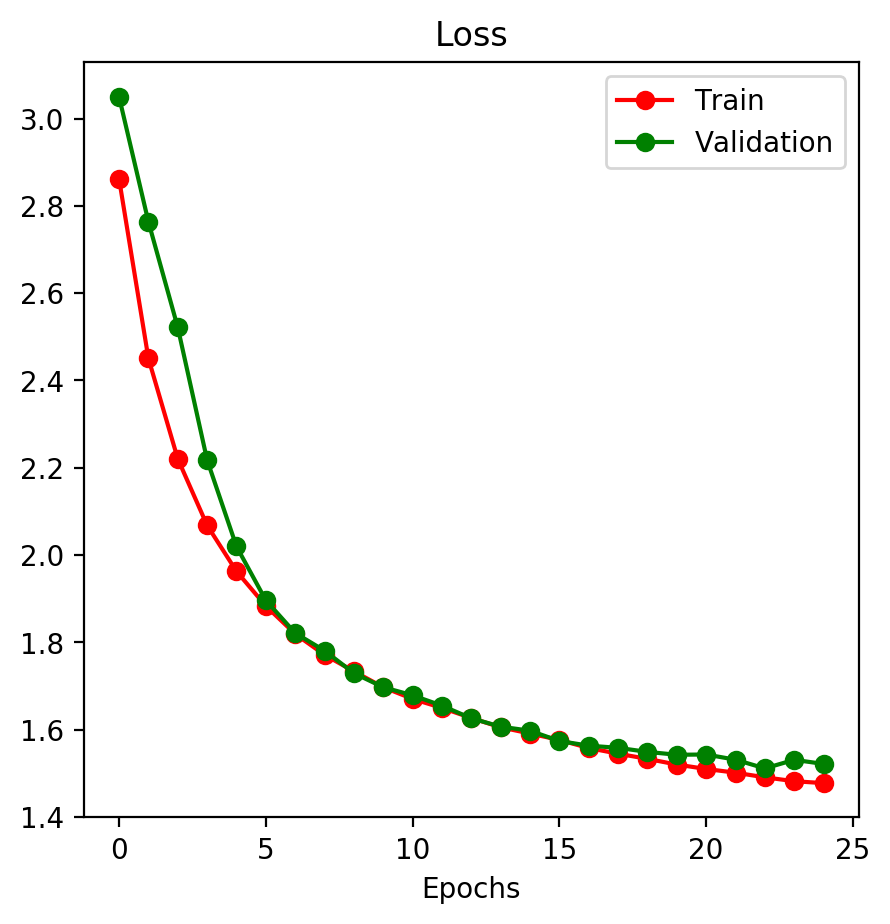
\includegraphics[width=\linewidth]{figures/partb_q2.png}
	\end{figure}
	
	\paragraph{Question 3}
	\begin{enumerate}[(i)]
		\item The coloured images are now more reasonable, the model with skip connections can now colour part of sky and grassland correctly.
		\item Skip connections successfully help improve performances. The validation loss reduces from 1.83 to 1.35 (-26\%), and the validation accuracy increases from 33\% to 49\%.
		\item The quality of coloured images is improved significantly compared with outcome of the previous CNN without skip connections.
		\item The model with skip connections has more trainable parameters than the previous CNN, it is more likely for it to pick up more complicated patterns.
		\item In the CNN without skip connections, the input to the very last convolution layer is an abstract representation of the original image. It could be that the representation is too abstract and the last convolution layer fails to infer colouring information from such an abstract representation. Adding skip connections helps the last convolution layer recall the previous information such as the raw image and activations of previous layers. In this case, the CNN with skip connections outperforms the vanilla CNN.
	\end{enumerate}
	\paragraph{Question 4} The training/validation loss and final images are included below. And the table below summarizes the validation loss and accuracy after 25 epochs. In most coloured pictures from models trained with small batch sizes (50 and 100), the colouring is finer and more accurate especially at edges of objects. Evaluating metrics suggest a smaller batch size helps improve both models' losses and accuracy on the validation set.
	
	\begin{table}[H]
		\centering
		\caption{Model Performances with Different Batch Sizes}
		\begin{tabular}{c|c c}
			\toprule
			Batch Size & Validation Loss & Validation Accuracy \\
			\midrule
			50 & 1.32 & 50\% \\
			100 & 1.36 & 49\% \\
			500 & 1.52 & 43\% \\
			1,000 & 1.63 & 41\% \\
			\bottomrule
		\end{tabular}
	\end{table}
	
	\begin{figure}[H]
		\centering
		\caption{Final Image Outputs with Batch Size = 50, 100, 500, 1000 (from top to bottom)}
		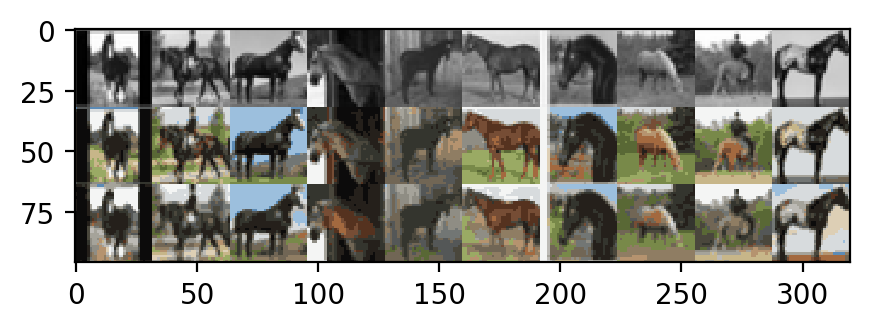
\includegraphics[width=\linewidth]{figures/unet_output_bs_50.png}
		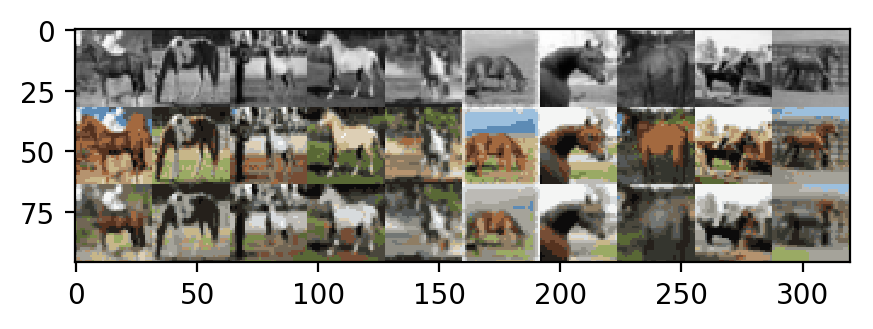
\includegraphics[width=\linewidth]{figures/unet_output_bs_100.png}
		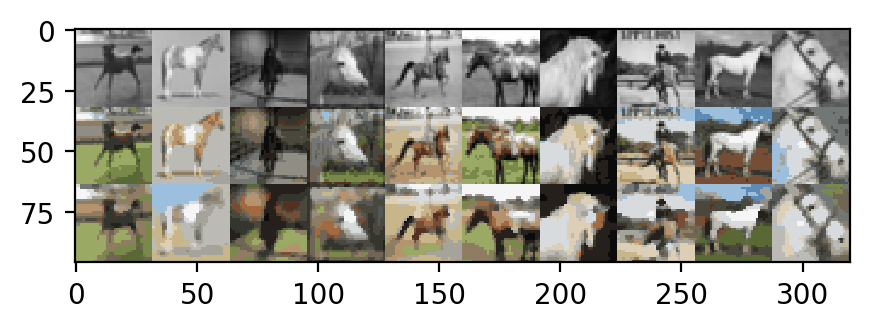
\includegraphics[width=\linewidth]{figures/unet_output_bs_500.png}
		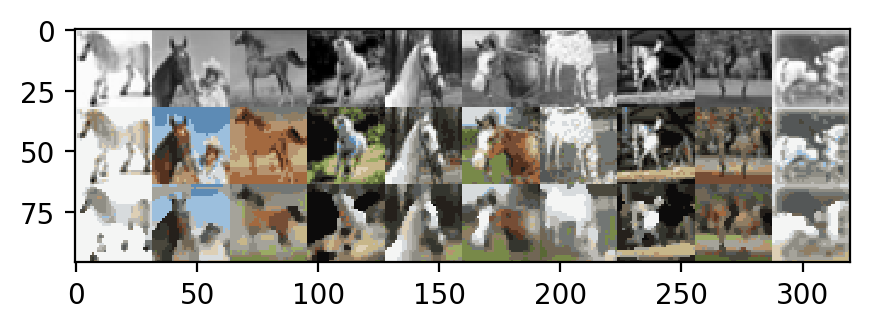
\includegraphics[width=\linewidth]{figures/unet_output_bs_1000.png}
	\end{figure}

	\begin{figure}[H]
		\centering
		\caption{Batchsize=50(left) and 100(right)}
		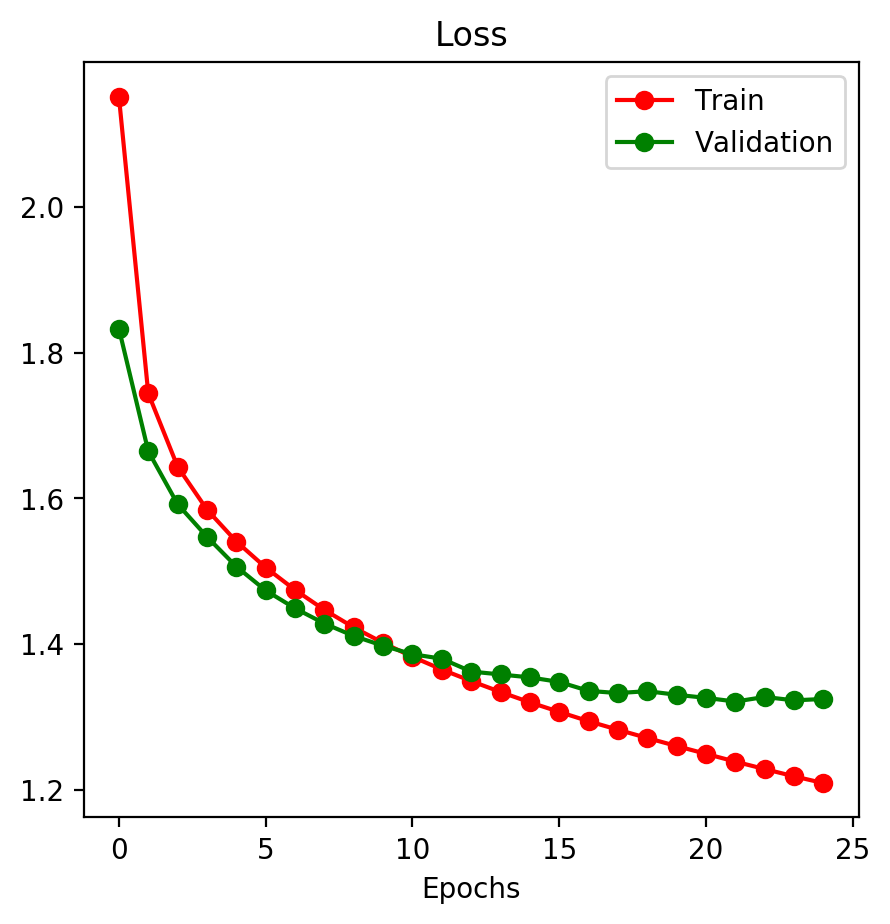
\includegraphics[width=0.45\linewidth]{figures/unet_learning_bs_50.png}
		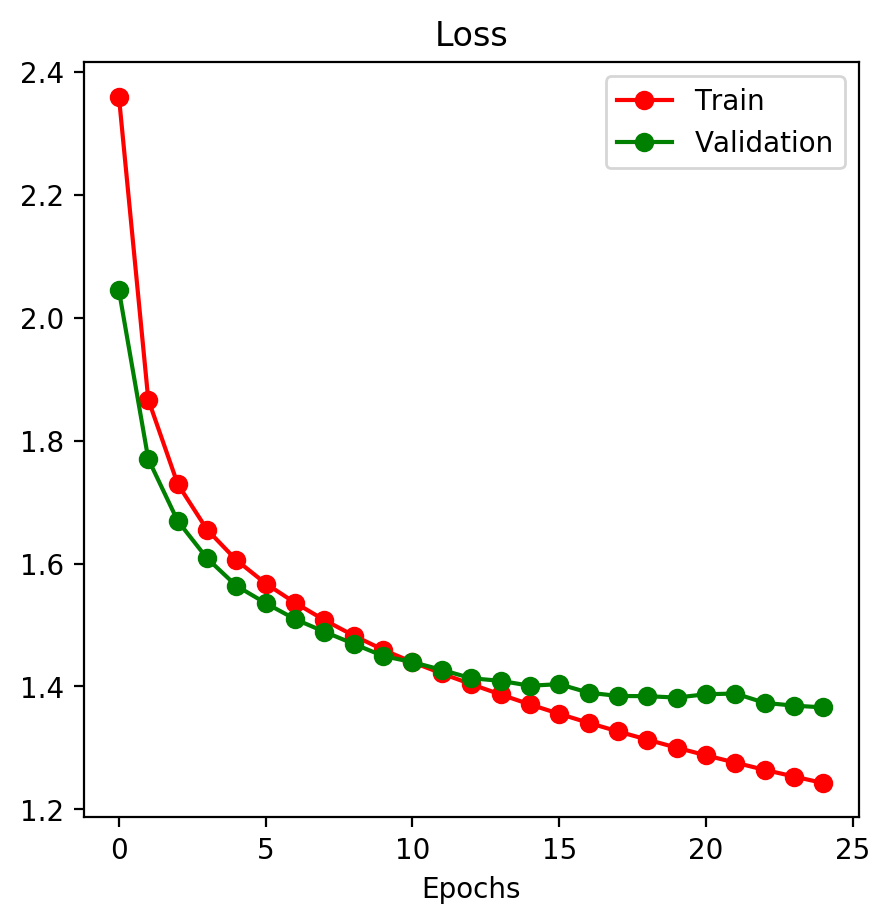
\includegraphics[width=0.45\linewidth]{figures/unet_learning_bs_100.png}
	\end{figure}

	\begin{figure}[H]
		\centering
		\caption{Batchsize=500(left) and 1,000(right)}
		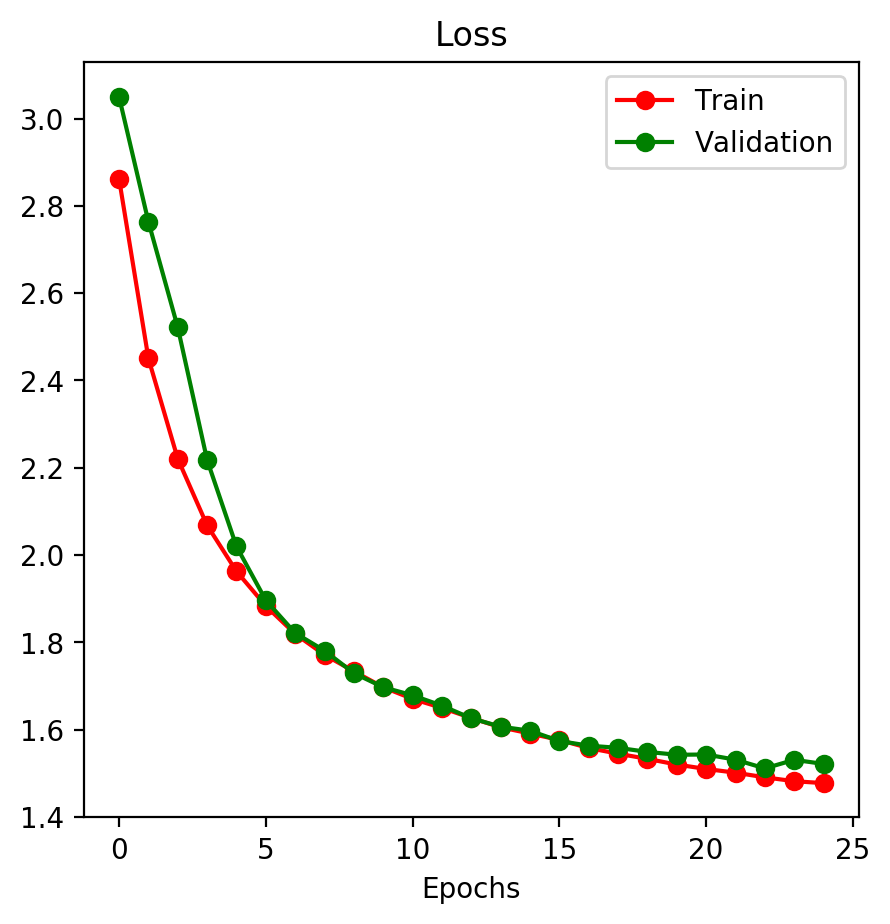
\includegraphics[width=0.45\linewidth]{figures/unet_learning_bs_500.png}
		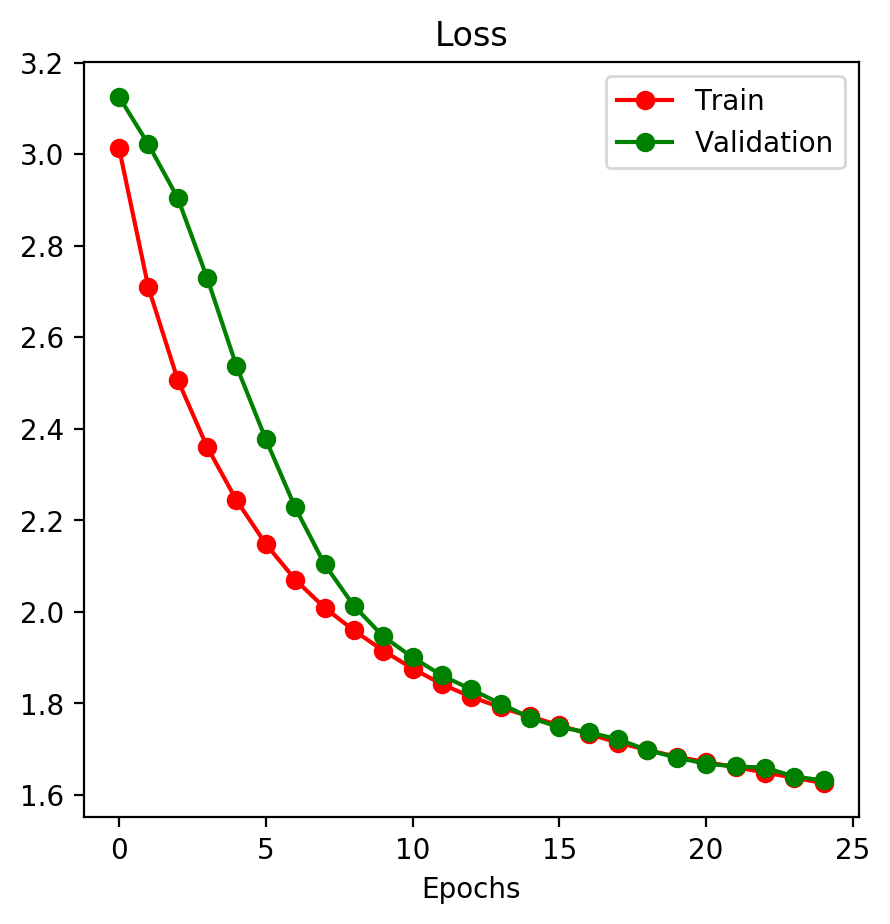
\includegraphics[width=0.45\linewidth]{figures/unet_learning_bs_1000.png}
	\end{figure}
	
	\section{Fine-tune Semantic Segmentation Model}
	\paragraph{Question 1} Implementation:
	\begin{lstlisting}[language=python]
for name, param in model.named_parameters():
    if name.startswith("classifier.4"):
        learned_parameters.append(param)
	\end{lstlisting}
	\paragraph{Question 2} Implementation:
	\begin{lstlisting}[language=python]
model.requires_grad_(False)
model.classifier[4] = nn.Conv2d(
	256, 21, kernel_size=(1, 1), stride=(1, 1)
)
	\end{lstlisting}
	
	\paragraph{Question 3} The visualized predictions:
	\begin{figure}[H]
		\centering
		\caption{Prediction on Training Set}
		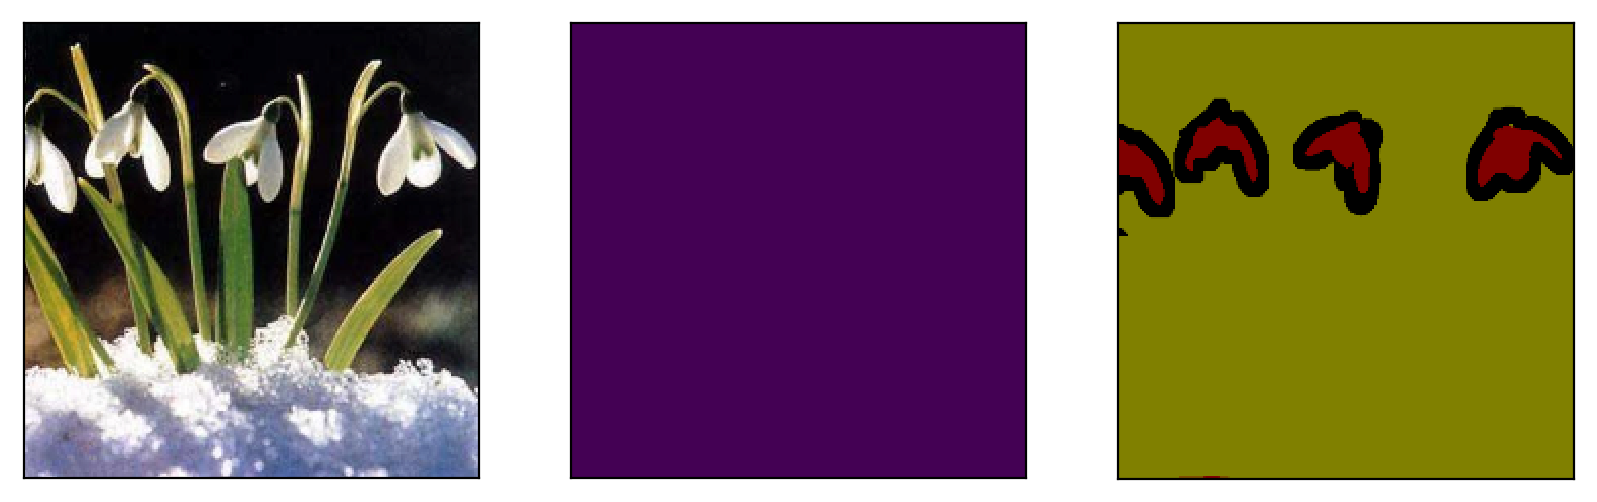
\includegraphics[width=\linewidth]{figures/train0.png}
		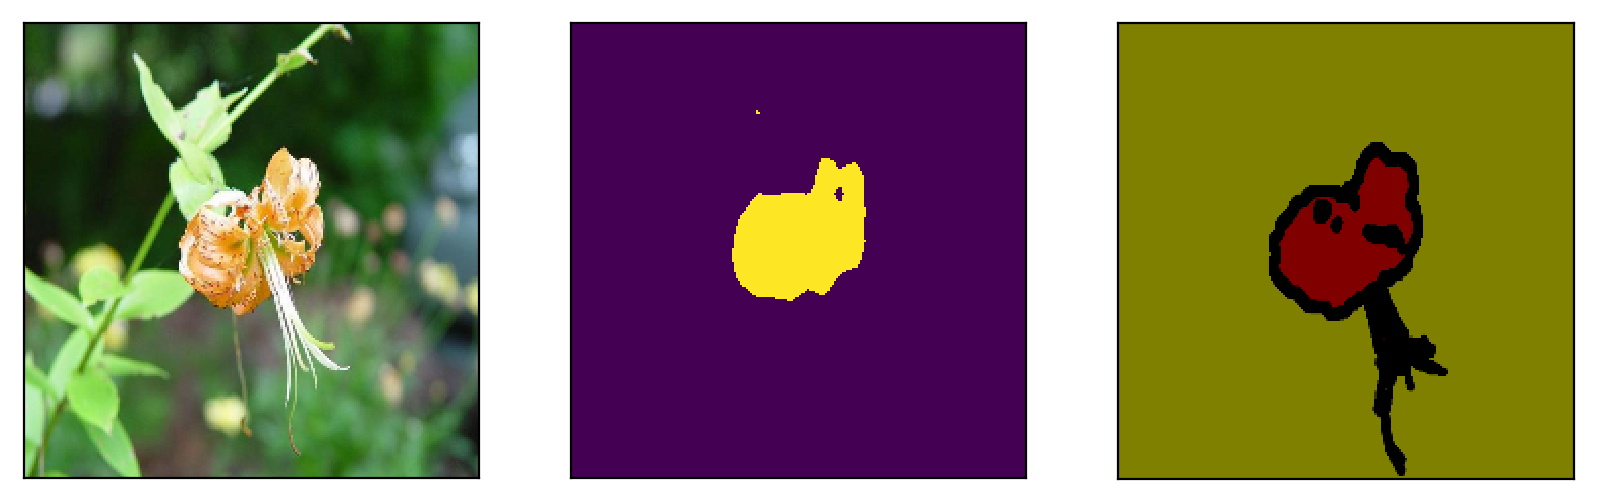
\includegraphics[width=\linewidth]{figures/train1.png}
		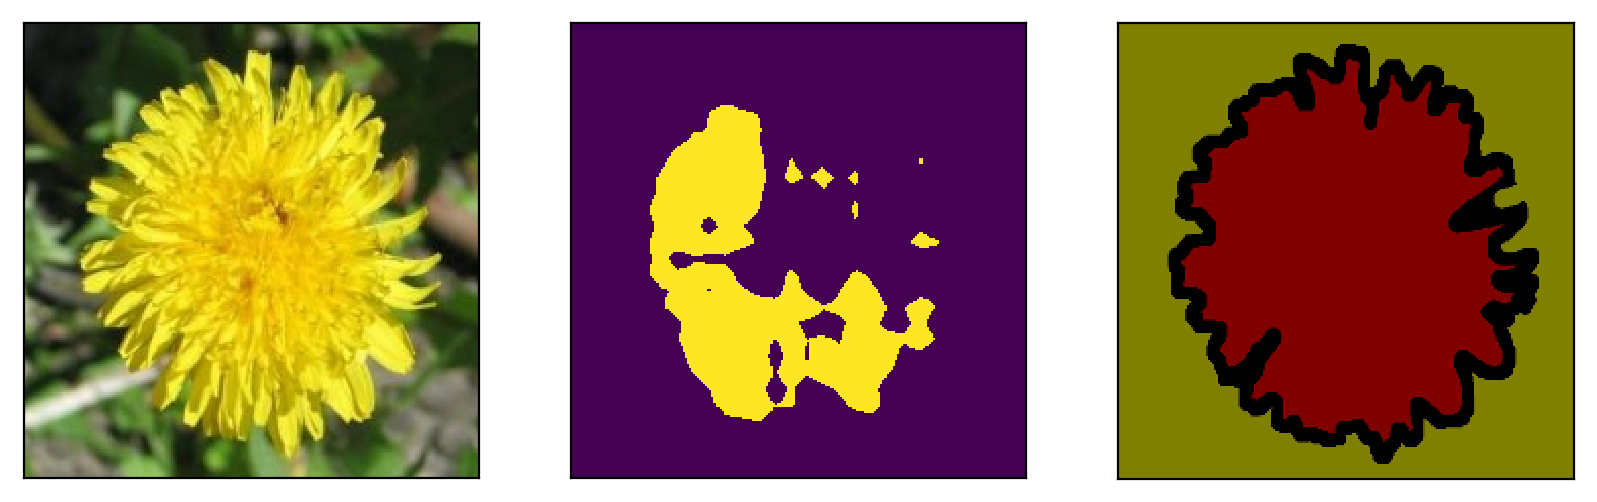
\includegraphics[width=\linewidth]{figures/train2.png}
		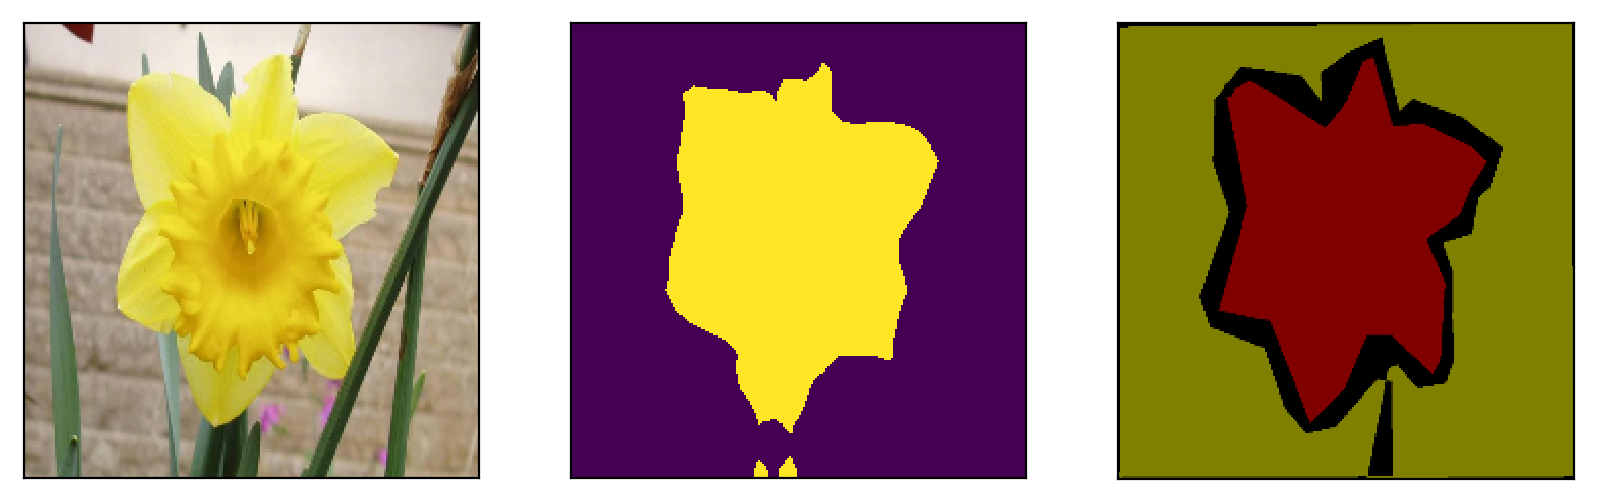
\includegraphics[width=\linewidth]{figures/train3.png}
	\end{figure}

	\begin{figure}[H]
		\centering
		\caption{Prediction on Validation Set}
		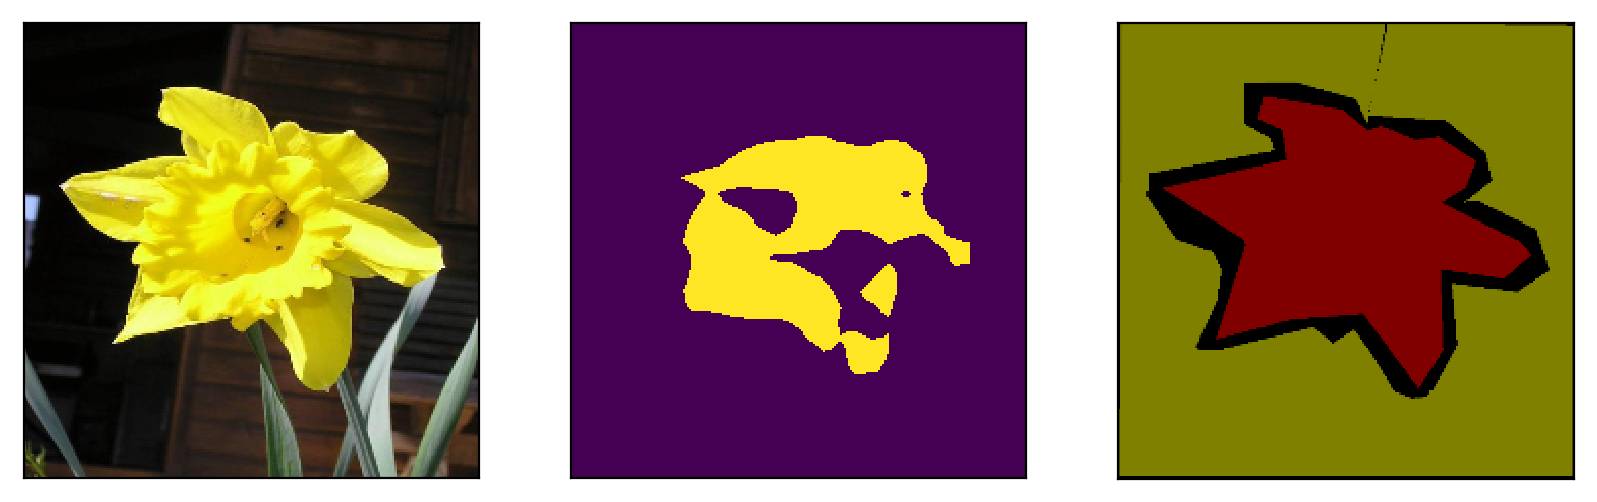
\includegraphics[width=\linewidth]{figures/val0.png}
		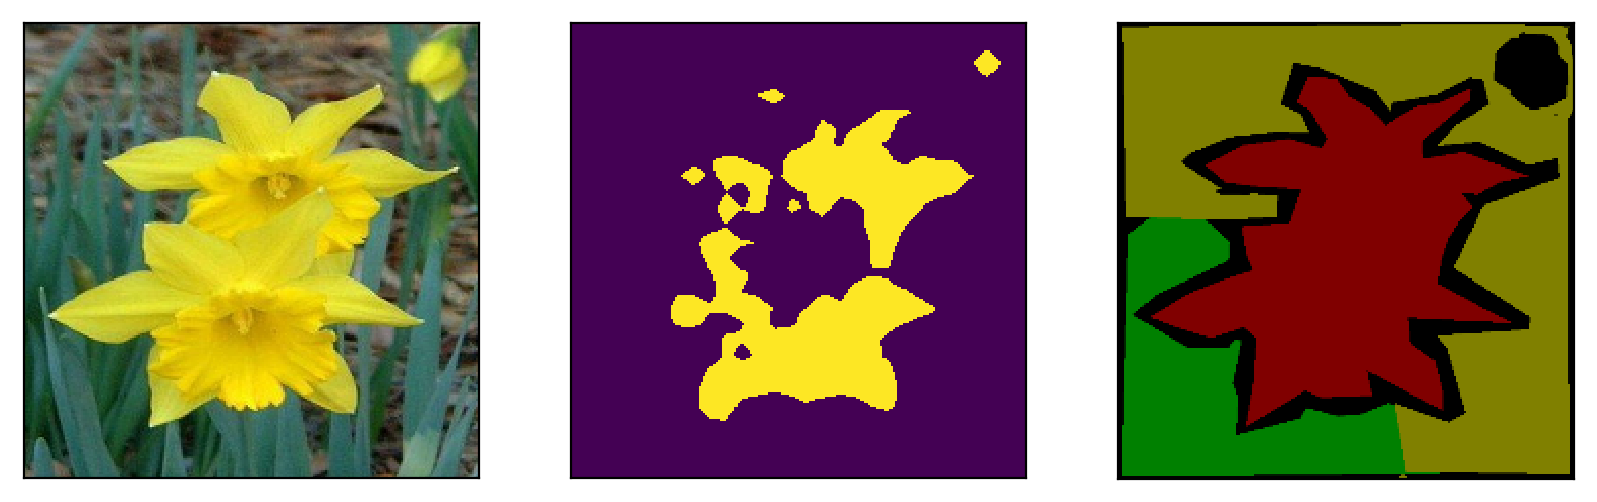
\includegraphics[width=\linewidth]{figures/val1.png}
		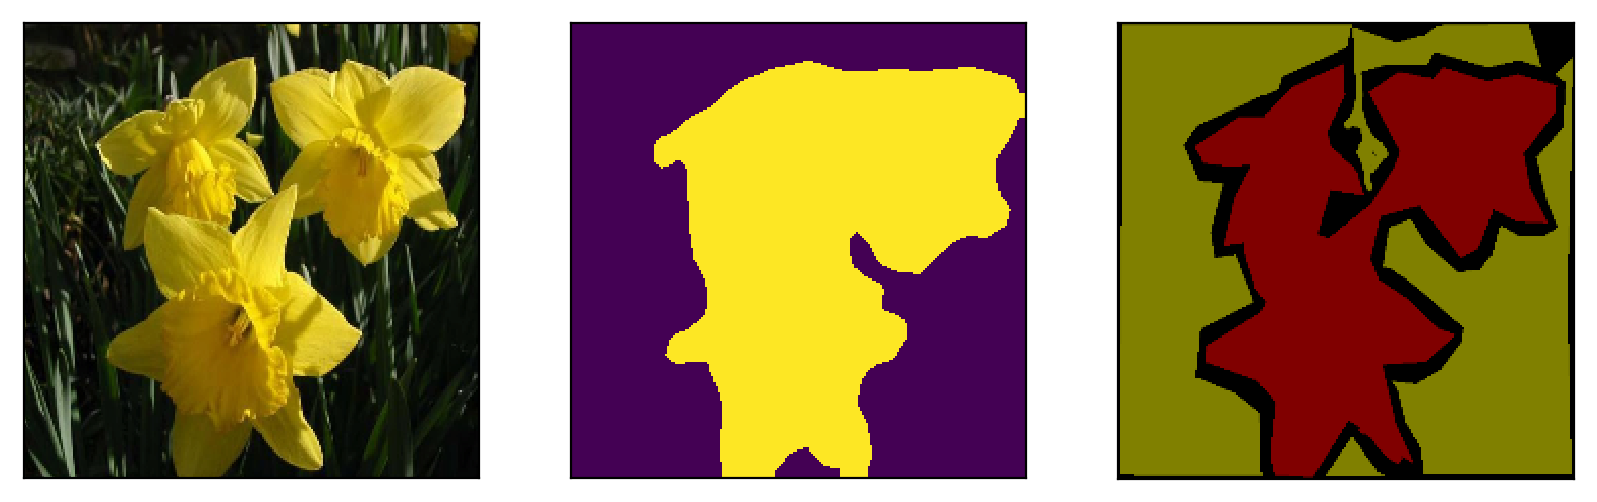
\includegraphics[width=\linewidth]{figures/val2.png}
		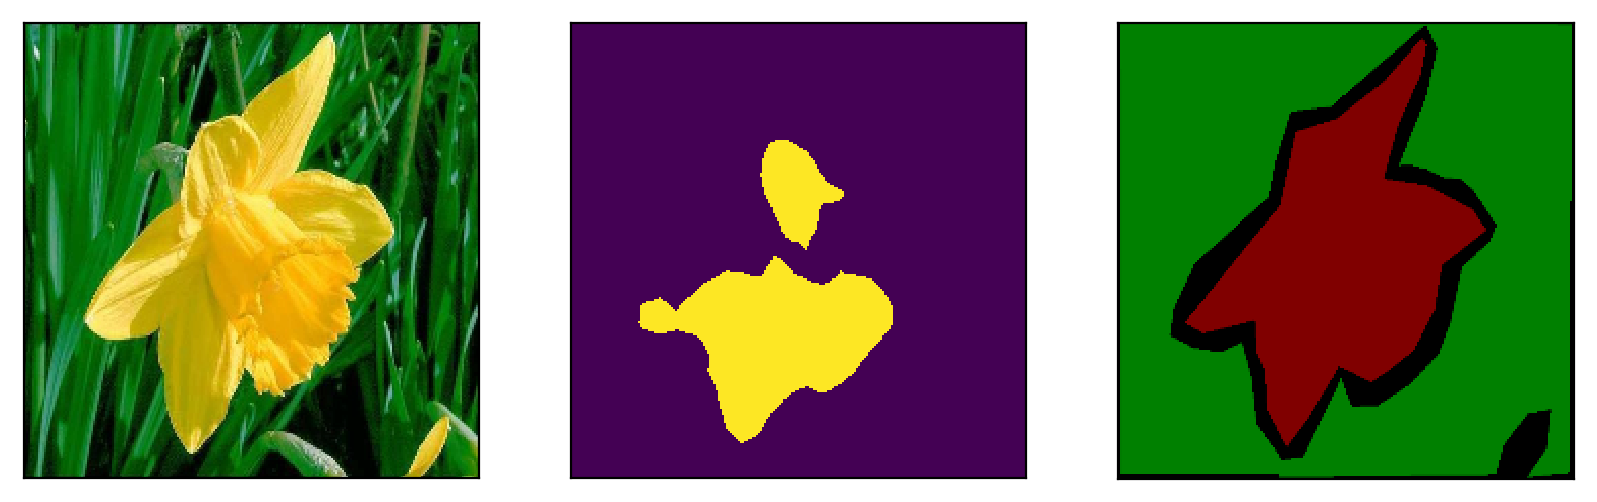
\includegraphics[width=\linewidth]{figures/val3.png}
	\end{figure}
	\paragraph{Question 4} \textbf{Memory Cost} The memory required of tuning the entire model involves storing all trainable parameters and the gradient with respect to each trainable parameter. If we are tuning the entire model, the activation of all layers must be stored so that we can compute the error signal (gradient of loss w.r.t. weights in hidden layer) of each layer during backward phase. Activations of hidden layers and gradient (in backward phase) takes memory cost at $\mc{O}(n)$. \\
	However, while tuning only the last layer, since we only need the error signal, only the activation of the last hidden layer is needed in the backward phase. Therefore, during the forward passing, the activation of the previous hidden layer can be discarded after the activation of current hidden layer is computed. The total memory cost of the forward phase is $\mc{O}(1)$. Similarly, we only need to store the gradient of loss w.r.t. weights in the last layer, the memory cost of backward phase is $\mc{O}(1)$ as well. \\
	The overall memory complexity of tuning the entire model is in $\mc{O}(n)$, and tuning only one layer is in $\mc{O}(1)$. \\
	\textbf{Computational Cost}
	While tuning only one layer, we only need computational power at $\mc{O}(1)$ to do backward propagation. Meanwhile, the computational cost of backward propagation for tuning the entire model is at $\mc{O}(n)$. 
	However, in both cases, we need to conduct the forward passing at a computational cost at $\mc{O}(n)$.
	Hence, tuning the entire model and tuning only one layer both have computational complexity of $\mc{O}(n)$.
	
	\paragraph{Question 5} The number of trainable parameters in each layer within this model only depends on kernel sizes, number of input channels and number of output channels. These numbers are unchanged when the size of input image changes. Therefore, the total number of parameters and memory needed to store the model is unchanged. \\
	However, the new dataset with larger images now requires 400\% memory, compared with the original dataset, to be stored.
\end{document}
























